\documentclass[11pt,a4paper, dvipdfmx]{article}

% margin
\usepackage[left=20mm,right=20mm,top=25.5mm,bottom=28.5mm,footskip=10mm,headsep=19pt]{geometry}

% packages
\usepackage{graphicx}
\usepackage{hyperref}
\usepackage{algorithmic}
\usepackage{booktabs}
\newcommand{\theHalgorithm}{\arabic{algorithm}}

% math macros
\usepackage{mymacros}

\title{テンプレート}
\author{masayoshi64}
\date{February 2024}

\begin{document}

\maketitle

\section{マクロ}
\[\R, \1, \Abb, \cA\]
\[\xhat, \xbar, \xtld\]
\[\argmin, \argmax\]
\[\veps, \vGam\]
\[\Expec[\mu]{X}, \Prob[\mu]{X \geq 0}, \Var[\mu]{X}\]
\[\pmx{
        a & b                \\
        c & d
    }\]
\[\dist, \proj, \conv, \iid, \vspan, \sign, \range \]
\[\psd{n}, \pd{n}\]
\[\kl{a}{b}, \opnorm{A}, \frobnorm{A}, \infnorm{B}, \set{a, b, c}, \floor{a}, \ceil{a}\]

\section{画像}
dvipdfmxオプションを使うのを忘れずに.
\begin{figure}[htbp]
    \centering
    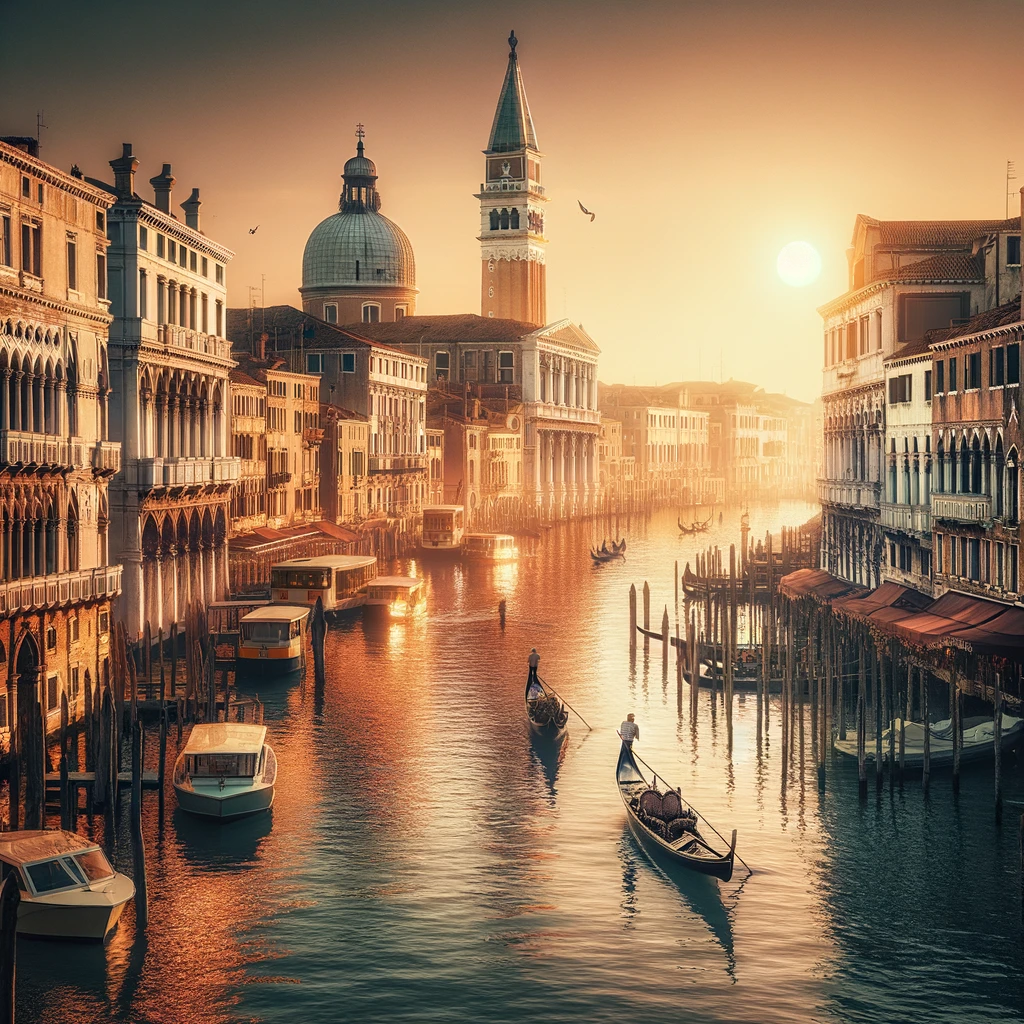
\includegraphics[width=0.5\textwidth]{figs/test.png}
    \caption{図1}
    \label{fig:fig1}
\end{figure}

\section{表}
booktabsパッケージを使う.
\begin{table}[h]
    \caption{表1}
    \label{table:table1}
    \centering
    \begin{tabular}{lcc}
        \toprule
        A  & B  & C  \\
        \midrule
        a  & b  & c  \\
        aa & bb & cc \\
        \bottomrule
    \end{tabular}
\end{table}

\section{引用}
\cite{jacot2018neural}によると...\\
...である~\cite{rafailov2023direct}.

\bibliography{main}
\bibliographystyle{plain}

\end{document}


